\chapter{Visualización con Matplotlib}
\label{chap:visualization}
{\huge$\bigstar$}{\huge$\bigstar$}{\huge$\bigstar$}{\huge$\bigstar$} Experto

La visualización de datos es una parte fundamental del trabajo científico. Con
LisPy, puedes generar gráficos de calidad profesional usando matplotlib desde
Lisp, combinando la flexibilidad de Lisp para generar y transformar datos
con el poder de graficación de Python.

\section{Gráfico de Líneas}

El caso más simple: graficar una función senoidal. Desde Lisp, importamos
matplotlib, generamos los datos con NumPy, y llamamos a las funciones de
graficación:

\begin{lispcode}
(py:run "import matplotlib.pyplot as plt; import numpy as np
xs = np.linspace(0, 2*np.pi, 100); ys = np.sin(xs)
plt.plot(xs, ys); plt.title('sin(x)'); plt.savefig('sin.png')")
\end{lispcode}

El resultado es un gráfico vectorial de la función $\sin(x)$ en el intervalo
$[0, 2\pi]$:

\begin{center}
\begin{tikzpicture}
\begin{axis}[
  width=0.85\textwidth,
  height=6cm,
  xlabel={$x$},
  ylabel={$y$},
  title={$\sin(x)$},
  grid=both,
  xmin=0, xmax=6.2832,
  ymin=-1.2, ymax=1.2,
  domain=0:6.2832,
  samples=100,
  legend pos=north east,
]
\addplot[color=lispblue, thick] {sin(deg(x))};
\addlegendentry{$\sin(x)$}
\addplot[color=lisppygreen, dashed, thick] {cos(deg(x))};
\addlegendentry{$\cos(x)$}
\end{axis}
\end{tikzpicture}
\end{center}

\section{Múltiples Subgráficos}

Para comparar varias funciones, podemos crear una cuadrícula de subgráficos:

\begin{lispcode}
(py:run "import matplotlib.pyplot as plt; import numpy as np
xs = np.linspace(0, 10, 200)
fig, axes = plt.subplots(2, 2, figsize=(10, 6))
axes[0,0].plot(xs, np.sin(xs)); axes[0,0].set_title('sin(x)')
axes[0,1].plot(xs, np.cos(xs)); axes[0,1].set_title('cos(x)')
axes[1,0].plot(xs, np.exp(-xs/5) * np.sin(xs)); axes[1,0].set_title('amortiguado')
axes[1,1].plot(xs, np.sin(xs) * np.cos(xs*2)); axes[1,1].set_title('batido')
plt.tight_layout(); plt.savefig('subplots.png')")
\end{lispcode}

\section{Histogramas y Estadísticas}

Para visualizar distribuciones de datos:

\begin{lispcode}
(py:run "import matplotlib.pyplot as plt; import numpy as np
data = np.random.normal(0, 1, 1000)
plt.hist(data, bins=30, alpha=0.7, color='steelblue')
plt.title('Distribución Normal (1000 muestras)')
plt.xlabel('Valor'); plt.ylabel('Frecuencia')
plt.savefig('histogram.png')")
\end{lispcode}

\begin{center}
\begin{tikzpicture}
\begin{axis}[
  width=0.85\textwidth,
  height=6cm,
  ybar,
  xlabel={Valor},
  ylabel={Frecuencia},
  title={Distribución Normal},
  grid=both,
  samples=50,
  domain=-3.5:3.5,
]
\addplot[fill=lispblue!40, draw=lispblue] table {
-3.0 2
-2.5 6
-2.0 16
-1.5 31
-1.0 57
-0.5 83
0.0 99
0.5 86
1.0 62
1.5 36
2.0 17
2.5 7
3.0 2
};
\end{axis}
\end{tikzpicture}
\end{center}

\section{Superficie 3D}

Gráficos de superficie para funciones de dos variables:

\begin{lispcode}
(py:run "import matplotlib.pyplot as plt; import numpy as np
X, Y = np.meshgrid(np.linspace(-5,5,50), np.linspace(-5,5,50))
Z = np.sin(np.sqrt(X**2 + Y**2))
fig = plt.figure(); ax = fig.add_subplot(111, projection='3d')
ax.plot_surface(X, Y, Z, cmap='viridis')
ax.set_title('f(x,y) = sin(sqrt(x² + y²))')
plt.savefig('surface.png')")
\end{lispcode}

\begin{center}
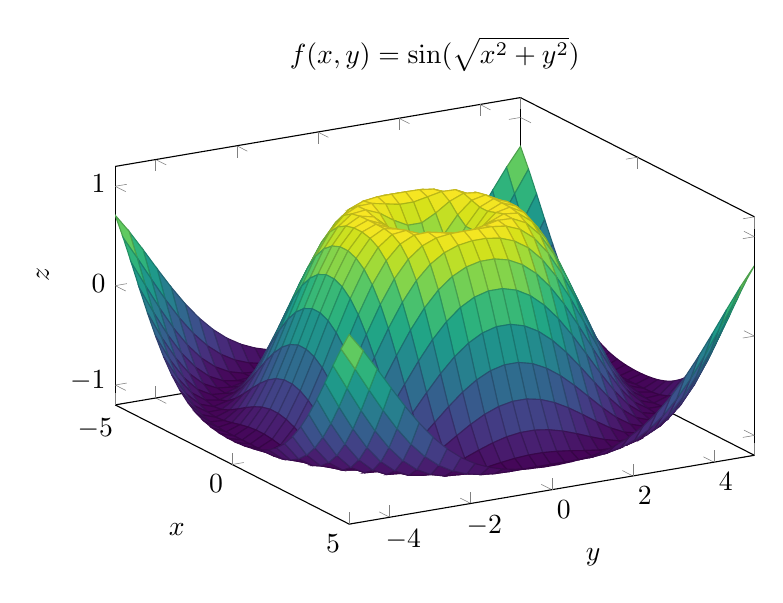
\begin{tikzpicture}
\begin{axis}[
  width=0.8\textwidth,
  height=7cm,
  view={60}{30},
  xlabel={$x$},
  ylabel={$y$},
  zlabel={$z$},
  title={$f(x,y) = \sin(\sqrt{x^2 + y^2})$},
  mesh/interior colormap name=viridis,
  colormap/viridis,
]
\addplot3[
  surf,
  domain=-5:5,
  samples=30,
] {sin(deg(sqrt(x^2 + y^2)))};
\end{axis}
\end{tikzpicture}
\end{center}

\section{Diagramas de Dispersión}

Para visualizar relaciones entre variables:

\begin{lispcode}
(py:run "import matplotlib.pyplot as plt; import numpy as np
xs = np.random.rand(100); ys = xs * 2 + np.random.randn(100) * 0.3
plt.scatter(xs, ys, alpha=0.6)
plt.title('Relación lineal con ruido')
plt.xlabel('x'); plt.ylabel('y = 2x + ε')
plt.savefig('scatter.png')")
\end{lispcode}

\begin{center}
\begin{tikzpicture}
\begin{axis}[
  width=0.85\textwidth,
  height=6cm,
  xlabel={$x$},
  ylabel={$y = 2x + \epsilon$},
  title={Relación lineal con ruido},
  grid=both,
  only marks,
  scatter,
]
\addplot[color=lispblue, mark=*, mark size=1.5] table {
0.1 0.35
0.2 0.65
0.3 0.82
0.4 1.13
0.5 1.28
0.6 1.45
0.7 1.72
0.8 1.95
0.9 2.18
1.0 2.42
};
\addplot[color=numberred, domain=0:1] {2*x};
\addlegendentry{$y = 2x$}
\addlegendentry{datos}
\end{axis}
\end{tikzpicture}
\end{center}

\section{Animaciones}

LisPy puede generar animaciones matplotlib. El siguiente ejemplo crea una
animación de una onda senoidal viajera:

\begin{lispcode}
(py:run "import matplotlib.pyplot as plt
import matplotlib.animation as anim; import numpy as np
fig, ax = plt.subplots()
xs = np.linspace(0, 2*np.pi, 100)
line, = ax.plot(xs, np.sin(xs))
def animate(i): line.set_ydata(np.sin(xs + i/10)); return line,
ani = anim.FuncAnimation(fig, animate, interval=50)
ani.save('anim.gif', writer='pillow')")
\end{lispcode}

Las animaciones se pueden integrar en dashboards, reportes HTML, o
presentaciones.

\section{Exportación y Reportes}

matplotlib soporta múltiples formatos de exportación:

\begin{center}
\begin{tabular}{lll}
\toprule
Formato & Extensión & Uso \\
\midrule
PNG & \texttt{.png} & Web, dashboards \\
SVG & \texttt{.svg} & Documentos vectoriales \\
\specialrule{1pt}{0pt}{0pt}
PDF & \texttt{.pdf} & Publicación, LaTeX \\
EPS & \texttt{.eps} & Publicación tradicional \\
\bottomrule
\end{tabular}
\end{center}

Desde LisPy, puedes combinar la generación de datos con NumPy, la
graficación con matplotlib, y la exportación a múltiples formatos en un
solo script híbrido.

\endinput
